\documentclass{article}
\usepackage{graphicx}
\usepackage[margin=1.5cm]{geometry}
\usepackage{amsmath}

\begin{document}
\twocolumn

\title{Warm Up: Energy I}
\author{Prof. Jordan C. Hanson}

\maketitle

\section{Memory Bank}

\begin{itemize}
\item $W = \vec{F} \cdot \Delta \vec{x}$ ... Definition of work
\item $U = mgh$ ... Work done against gravity in lifting an object of mass $m$ a distance $h$.
\item $P = \Delta E / \Delta t$ ... Definition of power.
\item $P = \vec{F} \cdot \vec{v}$ ... \textit{Instantaneous power} at constant velocity.
\item 1 hp (horsepower) is 735.5 Watts.
\item Conservative force: the work done on a system is zero if the displacement is a \textbf{closed path.}
\item Conservative forces: $F(x) = -dU/dx$ ... The negative derivative of the potential energy is the force.
\end{itemize}

\section{Work and Energy, Power}

\begin{enumerate}
\item An 80-kg army trainee does pull-ups on a horizontal bar (Fig. \ref{fig:1}). It takes the trainee 0.8 seconds to raise the body 60 cm, and 90\% of his weight is lifted. How much power do the muscles supply moving his body? \\ \vspace{2cm}
\item (a) Calculate the power needed for a 950-kg car to climb a 5.0 degree slope at a constant 30.0 m s$^{-1}$ while encountering wind resistance and friction totaling 600 N. (b) Convert to horsepower. \\ \vspace{2cm}
\end{enumerate}

\section{Potential Energy and Conservative Forces}

\begin{enumerate}
\item \textbf{Potential energy of a hiker}, part 1.  Notice that the potential energy resulting from gravity is $U(y) = mgy + const$, because $\Delta U = mg\Delta y$.  (a) If $F = -\Delta U/\Delta y$, what is $F$? (b) Why can we add some constant to $U(y)$ without changing this? \\ \vspace{0.5cm}
\item \textbf{Potential energy of a hiker}, part 2.  Suppose we hike to the top of Hellman Park, just North of Whittier College.  (a) If the change in altitude is 150 m, and our mass is 90 kg, what is the change in potential energy? (b) If we walk around the peak of the hill without changing altitude, what is $\Delta U$? (c) If we base jump off a 150 m cliff into water, what is our final speed before we hit the ground? \\ \vspace{2.5cm}
\item Suppose we have a quadratic potential energy function: $U(x) = \frac{1}{2}k x^2$. (a) What is the associated conservative force? (b) Graph the function $U(x)$ below. (c) Show that the negative slope always points towards the origin.
\end{enumerate}

\begin{figure}
\centering
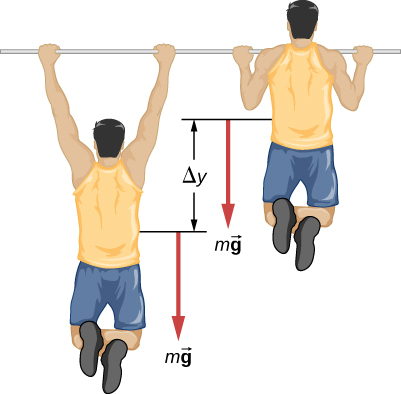
\includegraphics[width=0.33\textwidth]{figures/pull_up.jpeg}
\caption{\label{fig:1}}
\end{figure}


\end{document}
